\documentclass[catalan,border=15pt,class=scrartcl,multi=minipage,parskip=half*]{standalone}

% encoding
\usepackage[utf8]{inputenc}
\usepackage[T1]{fontenc}
\usepackage{lmodern}
\usepackage{babel}

% formatting and fixes
\frenchspacing
\usepackage[style=spanish]{csquotes}
\MakeAutoQuote{«}{»}
\usepackage{bookmark}

% ADD ANY SPECIFIC PACKAGES HERE
% (CHEMISTRY, CODE, PUBLISHING)
\usepackage[usenames,dvipsnames,svgnames,table]{xcolor}
\usepackage{adjustbox}
\usepackage{booktabs}
\usepackage{mathtools}
\usepackage{commath}
\usepackage{tikz}
\usepackage{siunitx}
\usepackage{nicefrac}
\usetikzlibrary{calc}
\usetikzlibrary{arrows.meta}
\usetikzlibrary{automata}
\usepackage{minted}

% other options
\setcounter{tocdepth}{6}
\setcounter{secnumdepth}{2}

% hyperlink setup / metadata
\usepackage{hyperref}
\AfterPreamble{\hypersetup{
  pdfauthor={Xavier Mendez},
  pdfsubject={IPAV},
  pdfpagelayout=OneColumn,
}}

% custom commands
\newcommand{\startpage}{\begin{minipage}{30em} \setlength{\parskip}{0.5em}}
\newcommand{\finishpage}{\end{minipage}}
\newcommand{\iopair}[2]{\( \left(#1\right) \rightarrow #2 \)}

\AfterPreamble{\hypersetup{
  pdftitle={Entregable 7: Interpolación},
}}

\begin{document}
\startpage

\paragraph{Problema 1.}

\subparagraph{Apartado A.} \hspace{1em}

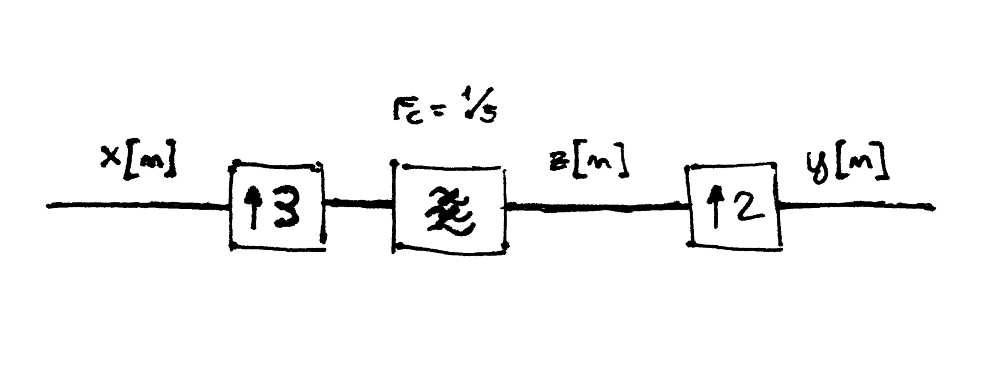
\includegraphics[width=\textwidth]{T7-p1a}

\subparagraph{Apartado B.}

Sea $B$ el ancho de banda discreto de la señal $x[n]$ (que, asumiendo que es
real, no puede ser superior a $\nicefrac{1}{2}$).

Una vez interpolada, la primera réplica de la señal empieza en
$\nicefrac{1}{3} - \nicefrac{B}{3}$. Por tanto, para que el filtro elimine
todas las réplicas debe cumplirse que $\nicefrac{1}{5} < \nicefrac{1}{3} -
\nicefrac{B}{3} \Leftrightarrow B < 1 - \nicefrac{3}{5} = \nicefrac{2}{5}$.

\subparagraph{Apartado C.}

Siguiendo las definiciones:
%
\begin{align*}
  Z(F) &= X(3F) \cdot H_0(F) \\
  Y(F) &= Z(2F) = X(6F) \cdot H_0(2F)
\end{align*}

\subparagraph{Apartado D.}

Si nos basamos en la segunda igualdad del apartado anterior, por inspección
simple sería equivalente a interpolar $x[n]$ por 6, y luego filtar con un
filtro discreto con respuesta $H_0(2F)$ (tengamos en cuenta que $H_0(F)$
es una función periódica por lo que «arrastramos» una réplica hacia
$F=\nicefrac{1}{2}$).

\finishpage
\startpage

\paragraph{Problema 2.}

\subparagraph{Apartado A y B.}

Queremos obtener una señal donde $X(F)$ habrá sido compactado por 6 (debido
a la nueva frecuencia de muestreo) y luego desplazado hacia $F_c = \pm \frac{
\SI{16}{\kilo\hertz}}{\SI{48}{\kilo\hertz}} = \pm \nicefrac{1}{3}$. Dado que
la señal de salida es real, también estaría replicada en $1 - \nicefrac{1}{3}
= \nicefrac{2}{3}$ (\SI{32}{\kilo\hertz}).

Teniendo esto en cuenta, la única opción que tiene sentido es que primero se
interpole con 2 y se filtre paso bajo a $f_c = \SI{4}{\kilo\hertz}$. Esto
dejaría una réplica de la señal en \SI{0}{\kilo\hertz}, \SI{16}{\kilo\hertz},
etc.

Luego se interpola con 3 y se filtra paso alto a $f_c = \SI{8}{\kilo\hertz}$.
Esto elimina las réplicas en \SI{0}{\kilo\hertz} y múltiplos, dejando solo
la de \SI{16}{\kilo\hertz} y sus reflejos.

\subparagraph{Apartado C.}

Al tratarse de señales reales, la parte negativa de las transformadas se ha
omitido por simplicidad.

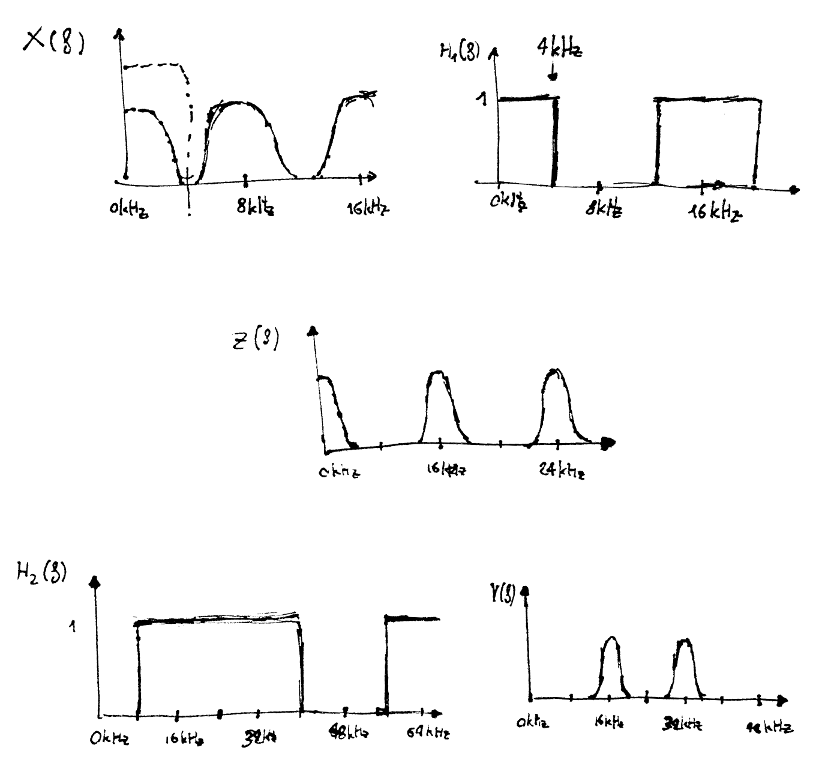
\includegraphics[width=\textwidth]{T7-p2c}

\finishpage
\startpage

\paragraph{Problema 3.}

\subparagraph{Apartado A.}

El ancho de banda discreto de la señal original es $B =
\frac{\SI{17}{\kilo\hertz}}{\SI{44.1}{\kilo\hertz}}$. Una vez interpolada,
la señal tendrá un ancho de banda de $\nicefrac{B}{4}$, y la primera réplica de
la señal empezará en la frecuencia $\nicefrac{1}{4} - \nicefrac{B}{4}$. Estos
valores son respectivamente $F_p$ y $F_a$. Si los calculamos aproximadamente:
%
\begin{align*}
  F_p \simeq \num{0.09637} \\
  F_a \simeq \num{0.15363}
\end{align*}

\subparagraph{Apartado B.}

Una vez filtrada, la señal interpolada solo tiene réplicas a $1 | F_p$.
El ancho de banda de la señal sigue siendo el mismo ($\nicefrac{B}{4}$,
\SI{17}{\kilo\hertz}), pero la primera réplica de la señal está ahora a
$1 - \nicefrac{B}{4}$, lo cual son \SI{159.4}{\kilo\hertz}. Estas dos
frecuencias son, respectivamente, $f_p$ y $f_a$ del filtro reconstructor.

\finishpage
\startpage

\paragraph{Problema 4.}

\subparagraph{Apartado A.} \hspace{1em}

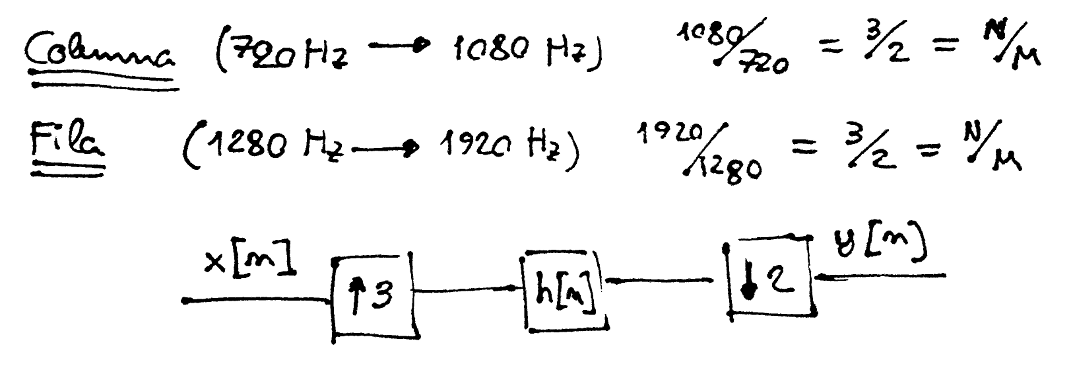
\includegraphics[width=\textwidth]{T7-p4a}

\subparagraph{Apartado B.}

Una vez interpolado, hay una muestra cada 3 muestras. Para que haya
interpolación lineal, $h[n]$ debería ser un pulso triangular de 6 muestras de
ancho: $h[n] = \Delta(\nicefrac{n}{3})$

\finishpage
\end{document}
